\documentclass{beamer}
\mode<presentation>
\usetheme{CambridgeUS}
\usepackage[russian]{babel}
\usepackage[utf8]{inputenc}
\usepackage[T2A]{fontenc}
\usepackage{sansmathaccent}

\usepackage{verbatim}
\usepackage{alltt}
\usepackage{minted}

\pdfmapfile{+sansmathaccent.map}
\title[Язык C]{Сигналы, каналы}
\author{Наумов Д.А., доц. каф. КТ}
\date[15.10.2019] {Операционные системы и системное программное обеспечение, 2019}

\begin{document}

%ТИТУЛЬНЫЙ СЛАЙД
\begin{frame}
  \titlepage
\end{frame}
  
%СОДЕРЖАНИЕ ЛЕКЦИИ
\begin{frame}
  \frametitle{Содержание лекции}
  \tableofcontents  
\end{frame}

\section{Сигналы}
\subsection{Введение}

\begin{frame}{Введение}
    Сигнал (программное прерывание) -— это оповещение процесса о том, что произошло некое событие. Такие события могут происходить из-за пределов системы -– например, из-за введения пользователем символа прерывания –- или возникать вследствие действий в программе или ядре.
    
    Один процесс может отправить сигнал другому процессу. При таком использовании сигналы могут рассматриваться как технология синхронизации и являются примитивной формой межпроцессного взаимодействия.
\end{frame}

\begin{frame}{Введение}
    Ядро отправляет процессу сигнал в следующих случаях
    \begin{itemize}
        \item Произошло аппаратное исключение. Это значит, что аппаратное обеспечение зафиксировало неверное состояние и оповестило об этом ядро, которое направило соответствующий сигнал затронутому процессу.
        \item Пользователь ввел один из специальных символов терминала, генерирующих сигналы.
        \item Произошло программное событие. Например, появился ввод из файлового дескриптора, сработал таймер, был завершен дочерний процесс.
    \end{itemize}
\end{frame}

\begin{frame}{Обработка сигнала}
    При получении сигнала процесс может выполнить следующие действия
    \begin{itemize}
        \item Игнорировать сигнал. Никакое действие не предпринимается. Существуют два сигнала, которые не могут быть проигнорированы: \texttt{SIGKILL} и \texttt{SIGSTOP}.
        \item Выполнить действие по умолчанию. Это действие зависит от того, какой сигнал отправляется.
        \item Вызвать обработчик сигнала. Ядро приостанавливает исполнение текущего кода процесса и переходит к ранее зарегистрированной функции. Затем процесс исполняет эту функцию. После выполнения обработчика, он переходит обратно в то место, где находился на тот момент, когда был захвачен сигнал.
    \end{itemize}
\end{frame}

\begin{frame}{Действия по умолчанию}
    По получении сигнала процесс по умолчанию выполняет одно из действий
    \begin{itemize}
        \item Сигнал игнорируется, то есть сбрасывается ядром и не влияет на процесс.
        \item Процесс завершается. Иногда это называют аварийным завершением процесса.
        \item Генерируется файл дампа ядра, и процесс завершается.
        \item Процесс останавливается.
        \item Выполнение процесса возобновляется.
    \end{itemize}
\end{frame}

\begin{frame}{Некоторые сигналы и действия по умолчанию}
    \begin{figure}
        \centering
        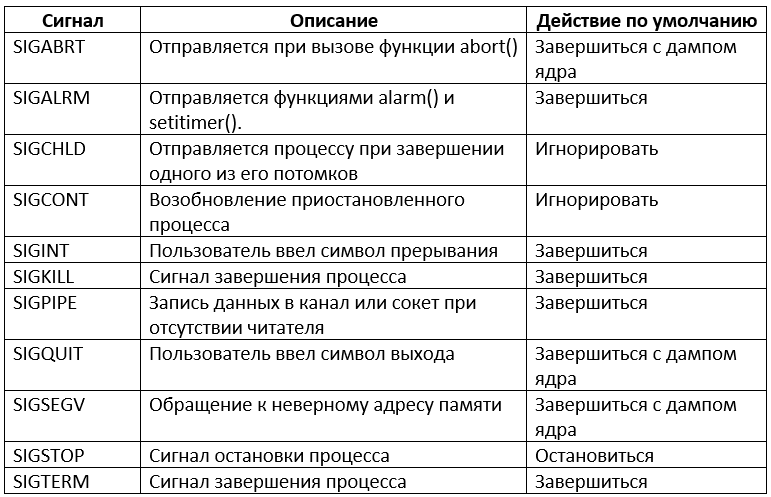
\includegraphics[scale=0.55]{signals-4.png}
    \end{figure}
\end{frame}

\subsection{Отправка сигналов}

\begin{frame}[fragile]{Отправка сигналов}
    Один процесс может отправить сигнал другому процессу с помощью системного вызова \texttt{kill()}.

\begin{minted}{c}
#include <signal.h>
int kill(pid_t pid, int sig);
// Возвращает 0 при успешном завершении 
// и –1 при ошибке
\end{minted}

    Аргумент \texttt{pid} идентифицирует один или несколько процессов, в которые отправляется сигнал \texttt{sig}.
    \begin{itemize}
        \item pid > 0 -- сигнал отправляет процессу с идентификатором pid.
        \item pid = 0 -- сигнал отправляется всем процессам группы, которой принадлежит вызывающий.
        \item pid < -1 -- сигнал отправляется всем процессам группы, идентификатор которой равен абсолютному значению pid.
        \item pid = -1 -- сигнал отправляется всем процессам, которым вызывающий процесс может отправлять сигналы (кроме init и самого себя).
    \end{itemize}
\end{frame}

\begin{frame}{Блокирование сигналов}
    Для каждого процесса ядро хранит сигнальную маску — набор сигналов, доставка которых в процесс временно заблокирована. Если в процесс отправляется заблокированный сигнал, то доставка этого сигнала откладывается до тех пор, пока сигнал не будет разблокирован путем удаления из сигнальной маски процесса. 
\end{frame}

\begin{frame}[fragile]{Блокирование сигналов}
    Системный вызов \texttt{sigprocmask()} может использоваться для добавления и удаления сигналов из сигнальной маски.
\begin{minted}{c}
#include <signal.h>
int sigprocmask(int how, const sigset_t *set, 
                sigset_t *oldset);
// Возвращает 0 при успешном завершении или –1 при ошибке
\end{minted}
    Аргумент \texttt{how} определяет, как изменится сигнальная маска
    \begin{itemize}
        \item \texttt{SIG\_BLOCK} -- сигналы, переданные в аргументе \texttt{set} будут включены в сигнальную маску.
        \item \texttt{SIG\_UNBLOCK} -- сигналы, переданные в аргументе \texttt{set} будут исключены из сигнальной маски.
        \item \texttt{SIG\_SETMASK} -- сигнальной маской станут сигналы, указанные в аргументе \texttt{set}.
    \end{itemize}
\end{frame}

\begin{frame}[fragile]{Наборы сигналов}
    Набор сигналов \texttt{sigset\_t} инициализируется функцией \texttt{sigemptyset()} или \texttt{sigfillset()}.
\begin{minted}{c}
#include <signal.h>
int sigemptyset(sigset_t *set);
int sigfillset(sigset_t, *set);
// возвращают 0 при успешном завершении или –1 при ошибке
\end{minted}

    Для добавления и удаления сигналов из набора используются функции \texttt{sigaddset()} и \texttt{sigdelset()}.
\begin{minted}{c}
#include <signal.h>
int sigaddset(sigset_t *set, int sig);
int sigdelset(sigset_t *set, int sig);
// возвращают 0 при успешном завершении или –1 при ошибке
\end{minted}
\end{frame}

\subsection{Обработка сигналов}

\begin{frame}[fragile]{Задание обработчиков}
    Обработчик сигнала -- это функция, вызываемая при получении указанного сигнала процессом.
    
    Функция \texttt{sigaction()} позволяет устанавливать и получать обработчик сигнала.
\begin{minted}{c}
#include <signal.h>
int sigaction(int sig, const struct sigaction *act, 
              struct sigaction *oldact);
// Возвращает 0 при успешном завершении или –1 при ошибке
\end{minted}

    Аргумент \texttt{sig} означает сигнал, для которого устанавливается обработчик.
    
    Аргумент \texttt{act} описывает политику обработки сигнала.
    
    После установки нового обработчика, старый будет записан в \texttt{oldact}.
\end{frame}

\begin{frame}[fragile]{Структура \texttt{sigaction}}
    Важными полями в структуре \texttt{sigaction} являются следующие
\begin{minted}{c}
struct sigaction {
    void (*sa_handler)(int);
    sigset_t sa_mask;
    int sa_flags;
};
\end{minted}
    
    \begin{itemize}
        \item \texttt{sa\_handler} -- обработчик сигнала
        \item \texttt{sa\_mask} --  сигналы, блокируемые во время вызова обработчика 
        \item \texttt{sa\_flags} -- параметры, контролирующие обработку сигнала
    \end{itemize}
\end{frame}

\subsection{Ожидание сигнала}

\begin{frame}[fragile]{Ожидание сигнала}
    Вызов функции \texttt{pause()} приостанавливает выполнение процесса до тех пор, пока он не получит сигнал.
\begin{minted}{c}
#include <unistd.h>
int pause(void);
// Всегда возвращает –1 с установкой errno в EINTR
\end{minted}
\end{frame}

\end{document}